% statistics_and_probability:x06 GDC:NO
\begin{question}
  \hspace*{\fill} [Note maximale: 5]\par
  \medskip

  \noindent Une scientifique étudie 100 poissons femelles et 100 poissons mâles. Elle mesure 
  leur longueur (arrondie au centimètre le plus proche). Les résultats sont donnés dans
  les diagrammes à boîtes et moustache suivants.\par
  \medskip

  \noindent Poissons femelles\par
  \medskip

  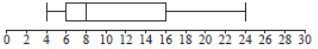
\includegraphics[scale=0.7]{poissons_femelles}\par  
  \medskip

  \noindent Poissons mâles\par
  \medskip

  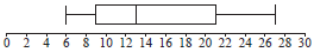
\includegraphics[scale=0.7]{poissons_males}\par  
  \medskip

  (a) Trouvez l’étendue des longueurs de tous les 200 poissons.\hspace*{\fill} [3]\par
  \medskip

  \noindent Quatre courbes de fréquence cumulée sont représentées ci-dessous.\par
  \medskip

  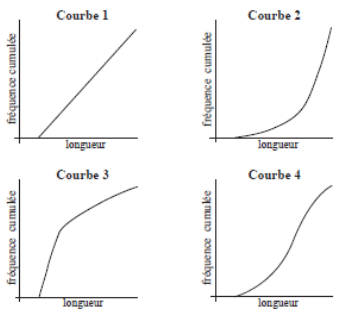
\includegraphics[scale=0.7]{courbe_1_a_4}\par  
  \medskip
  (b) Quelle courbe représente le mieux les longueurs des poissons femelles ?\hspace*{\fill} [2]\par  
\end{question}

